\documentclass[../../thesis.tex]{subfiles}

\begin{document}
\section{Pelegrin's works}

As stated in \cite{pelegrin-2023}, aircraft can be assumed to follow a well-defined \textit{network track}, which provides an internal structure to UAM corridors.  
Based on this, we can model UAM corridors using a directed graph, where the nodes represent either vertiports or cruise-level nodes.  
By \textit{cruise-level nodes}, we refer to nodes corresponding to take-off and landing pads, as well as intersections of different tracks.  
Since we are considering tactical deconfliction over a short time horizon, we assume that the graph remains static throughout the process.  

The model presented in the paper enforces a minimum safe distance that must be maintained between two aircraft, distinguishing between \textit{trailing} and \textit{non-trailing} conflicts.  
\begin{itemize}
    \item A \textbf{trailing conflict} occurs when two aircraft are on the same edge and must maintain at least $D$ units of separation.  
    \item A \textbf{non-trailing conflict} arises when two flights share a common source or destination node.  
\end{itemize}  

Since the speed of a flight is constant along an edge, conflicts need to be analyzed only at the relevant nodes.  
Non-trailing conflicts can be classified into three categories, illustrated in Figure \ref{fig:conflicts}:  
\begin{itemize}
    \item \textbf{Merging}: both aircraft enter the same node $x$.  
    \item \textbf{Diverging}: one aircraft enters and another exits from the same node $x$.  
    \item \textbf{Splitting}: both aircraft exit from the same node $x$.  
\end{itemize}  

To resolve these conflicts, different strategies must be applied depending on the type of interaction, while also considering the relative angles between aircraft to ensure a minimum separation of $D$ units.  
The proposed model optimizes the timing at which each flight occupies a node, ensuring compliance with speed constraints, minimizing total deviation at each node, and reducing delays for high-priority traffic.%
%As stated in \cite{pelegrin-2023}, aircraft can be assumed to follow a well-defined \textit{network track}, which provides an internal structure to UAM corridors.
%In this way, we can use direct graph to model the UAM corridors, more specifically the nodes of the graph will be veliports or cruise level nodes.
%With cruise level nodes we indicate the one node per take-off and one per landing pad and the intersection of the different tracks.
%Since we're considering a tactical deconfliction with short time horizon, we consider that the graph don't change during the process.
%The model presented in the paper consider a minimum safe distance that must be kept between two aircraft, for trailing and non-trailing conflicts.
%The first one happens when there are two aircraft in the same edge and they have to maintain at least $D$ units of distance.
%The second one happens when two flight have a source or destination node in common.
%We can classify the non-trailing conflict in three different groups, that can be visualized in Figure \ref{fig:conflicts}:
%\begin{itemize}
%    \item \textbf{Merging}, if both aircraft enter in the same node $x$
%    \item \textbf{Diverging}, if one aircraft enter and one exit from the same node $x$
%    \item \textbf{Splitting}, if both aircraft exit from the same node $x$
%\end{itemize}
%To consider this, we have to consider a different way to solve each type of conflict, and consider also the angle between the two aircraft, in order to maintain a distance at least of $D$ units of distance.
%In the model we try to find the safe time to stay in each node for each flight, maintaining the speed limits request, minimizing the total deviation and the delay for prior traffic. 
\begin{figure}

\centering
\begin{subfigure}{0.3\textwidth}
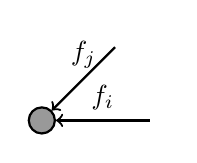
\begin{tikzpicture}[node distance={15mm}, thick]
\node[circle, draw=black, fill=black!40] (1) {}; 
\node[] (2)[right of=1]{};
\node[] (3)[above right of =1]{};

\draw [<-] (1) -- node[midway, above] {$f_i$} (2); 
\draw [<-] (1) -- node[midway, above] {$f_j$} (3);

\end{tikzpicture} 
\label{graph:merging}
\caption{Merging conflicts}
\end{subfigure}
\hfill
\begin{subfigure}{0.3\textwidth}
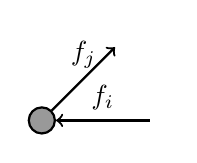
\begin{tikzpicture}[node distance={15mm}, thick, main/.style = {draw, circle}] 
\node[circle, draw=black, fill=black!40] (1) {}; 
\node[] (2)[right of=1]{};
\node[] (3)[above right of =1]{};

\draw [<-] (1) -- node[midway, above] {$f_i$} (2); 
\draw [->] (1) -- node[midway, above] {$f_j$} (3);

\end{tikzpicture} 
\caption{Diverging conflicts}
\label{graph:diverging}
\end{subfigure}
\hfill
\begin{subfigure}{0.3\textwidth}
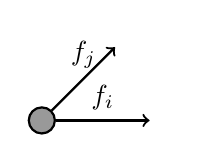
\begin{tikzpicture}[node distance={15mm}, thick, main/.style = {draw, circle}] 
\node[circle, draw=black, fill=black!40] (1) {}; 
\node[] (2)[right of=1]{};
\node[] (3)[above right of =1]{};

\draw [->] (1) -- node[midway, above] {$f_i$} (2); 
\draw [->] (1) -- node[midway, above] {$f_j$} (3);

\end{tikzpicture} 
\caption{Splitting conflicts}
\label{graph:splitting}
\end{subfigure}

\caption{The three different types of conflicts}
\label{fig:conflicts}
\end{figure}



\end{document}